
Given,
\begin{align}
F(x)= \begin{cases} 
       0  & if \:x<0\\
       \frac{x}{2} & if\: 0 \le x <1\\
       \frac{3}{5} & if \:1 \le x <2\\
       \frac{1}{2} +\frac{x}{8} & if\: 2\le x <3\\
       1  & if\: x\ge 3
    \end{cases} \label{a}
\end{align}
We need to find $\pr{2\le x <4}$,which is also can be written as
\begin{align}
\pr{2\le x <4} &= \pr{x<4} - \pr{ x <2}\\
              &= F(X=4^{-}) - F(X=2^{-})\label{b}
 \end{align} 
 Using \eqref{a} in \eqref{b},
 \begin{align}
 \pr{2\le x <4} &= 1 - \frac{3}{5}\\
                &= \frac{2}{5}\\
                &= 0.4 
\end{align} 


\begin{figure}[ht]
    \centering
    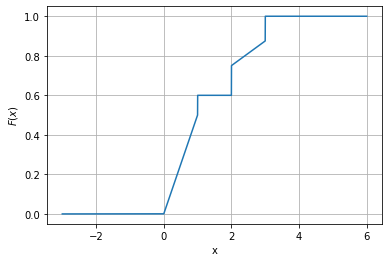
\includegraphics[width=\columnwidth]{solutions/adv/ma/2015/9/Fig_assign_5.png}
    \caption{cdf of random variable X}
\end{figure}
